\documentclass{article}
\setlength{\parskip}{5pt} % esp. entre párrafos
\setlength{\parindent}{0pt} % esp. al inicio de un párrafo
\usepackage{amsmath} % mates
\usepackage[sort&compress,numbers]{natbib} % referencias
\usepackage{url} % que las URLs se vean lindos
\usepackage[top=25mm,left=20mm,right=20mm,bottom=25mm]{geometry} % márgenes
\usepackage{hyperref} % ligas de URLs
\usepackage{graphicx} % poner figuras
\usepackage[spanish]{babel} % otros idiomas

\author{Raul L.} % author
\title{Pr\'{a}ctica 2: Autómata Celular} %título
\date{\today}

\begin{document} % inicia contenido

\maketitle % cabecera


\section{Introducci\'{o}n}\label{intro} % sección y etiqueta



En la segunda práctica trabajamos con autómatas celulares en dos dimensiones, particularmente el famoso juego de la vida. El estado del autómata se representa con una matriz booleana (es decir, contiene ceros y unos). Cada celda es o viva (uno) o muerta (cero). En cada paso, la supervivencia de cada celda (verde) se determina a partir de los valores de sus ocho vecinos (amarillos)\citep{ejemplo}.

\begin{figure}[h]
     \centering
     \includegraphics[width=70mm]{IMAGENES/P2V.png}
        \caption{tomado de la práctica 2
    \url{https://satuelisa.github.io/simulation/p2.html}}
     \label{}
 \end{figure}


En los extremos de la matriz, las celdas simplemente tienen menos vecinos. Otra alternativa sería considerar el espacio como un torus — pareciendo una dona — donde el extremo de abajo se reune con el extremo de arriba al igual como los lados izquierdo y derecho, uno con otro.

La regla de supervivencia es sencilla: una celda está viva si exactamente tres vecinos suyos están vivos. Para comenzar, usamos números pseudoaleatorios como el estado inicial\citep{ejemplo}

\section{Objetivo}
El objetivo de la simulaci\'{o}n diseña y ejecuta un experimento con por lo menos 30 r\'{e}plicas para estimar la probabilidad de creaci\'{o}n de vida dentro de 50 iteraciones (es decir, que haya celdas vivas al final de la r\'{e}plica), usando niveles de 10, 15 y 20 para el tamaño de la malla y los niveles 0.2, 0.4, 0.6 y 0.8 para la probabilidad inicial de vida. Visualiza y tabula los hallazgos\citep{ejemplo}.


\section{C\'{o}digo}
En el siguiente c\'{o}digo se utilizaron secuencias for para realizar todo el objetivo propuesto en una sola ejecución.El c\'{o}digo base se sac\'{o} del repositorio de Elisa Schaeffer, se modific\'{o}, ya que se deben agregar diferentes tamaños de matrices, haciendo el mismo procedimiento con 30 repeticiones en diferentes niveles de probabilidad.

\\ Código en Phyton 
\\\url{https://github.com/satuelisa/Simulation/blob/master/BrownianMotion}\\
**Código creado en Python**\\
\url{https://github.com/Raullr28/Resultados/blob/main/P2/PRACTICA2.py}
\begin{verbatim}
import numpy as np 
from random import random
import matplotlib.cm as cm
import matplotlib.pyplot as plt

dur = 50
lim = 9
seq = 0
probabilidad=(0.2, 0.4, 0.6, 0.8)
dimension=(10, 15, 20)
repeticiones=(30)

def mapeo(pos,actual):
    fila = pos // dim
    columna = pos % dim
    return actual[fila, columna]

def paso(pos):
    fila = pos // dim
    columna = pos % dim
    vecindad = actual[max(0, fila - 1):min(dim, fila + 2),
                      max(0, columna - 1):min(dim, columna + 2)]
    return 1 * (np.sum(vecindad) - actual[fila, columna] == 3)

def nuevos_valores(dim,num):#hice función lo de generar inicio aleatorio por rep
    valores = [1 * (random() < p) for i in range(num)]
    actual = np.reshape(valores, (dim, dim))
    assert all([mapeo(x,actual) == valores[x]  for x in range(num)])
    return(valores, paso, actual)


if __name__ == "__main__":
    vivieron=[]
    murieron=[]
    for p in probabilidad :
        print( "Probabilidad:",p,)
        for dim in dimension:
            print(" dimensión:",dim,)
            num = dim**2
            contador_viv=0
            contador_mue=0
            for rep in range(repeticiones):
                valores, paso, actual = nuevos_valores(dim,num)
                #genera valores iniciales distintos por rep
                
                for iteracion in range(dur):
                    valores = [paso(x) for x in range(num)]
                    vivos = sum(valores)
                    if vivos == 0:
                        contador_mue += 1
                        break; # nadie vivo
                    if iteracion == (dur-1):
                        contador_viv += 1
                        
                    actual = np.reshape(valores, (dim, dim))
            print(contador_viv)
            print(contador_mue)
            contador_viv=((contador_viv*100)/(rep+1))
            contador_mue=((contador_mue*100)/(rep+1))
            print("contador_viv",contador_viv)
            print("contador_mue",contador_mue)
            vivieron.append(contador_viv)
            murieron.append(contador_mue)
    print(vivieron)
    print(murieron)

PB02=vivieron[0:3]
PB04=vivieron[3:6]
PB06=vivieron[6:9]
PB08=vivieron[9:12]
print("0.2",PB02)
print("0.4",PB04)
print("0.6",PB06)
print("0.8",PB08)
separacion = np.arange(3)
plt.plot(separacion,PB02,label='Nivel 0.2')
plt.scatter(separacion,PB02)
plt.plot(separacion,PB04,label='Nivel 0.4')
plt.scatter(separacion,PB04)
plt.plot(separacion,PB06,label='Nivel 0.6')
plt.scatter(separacion,PB06)
plt.plot(separacion,PB08,label='Nivel 0.8')
plt.scatter(separacion,PB08)
plt.xticks(separacion , ('10', '15', '20'))
plt.ylabel('supervivencia (%)')
plt.xlabel('Dimensiónes')
plt.title('Supervivencia de poblacion')
plt.legend()
plt.show()
\end{verbatim}


\newpage
% Computational Results
\section{Resultados}
En la figura se muestra como se comporta cada dimensión con un ciclo de 30 repeticiones, el color azul es el nivel 0.2, el color amarillo es el nivel 0.4, el color verde es el nivel 0.6 y el color rojo es el nivel 0.8. Se puede observar tanto en las tablas como en la imagen, que el porcentaje de población fue muy pequeño ya que en muchos de los casos el porcentaje de vivos fue 0 .

 \begin{figure}[h]
     \centering
     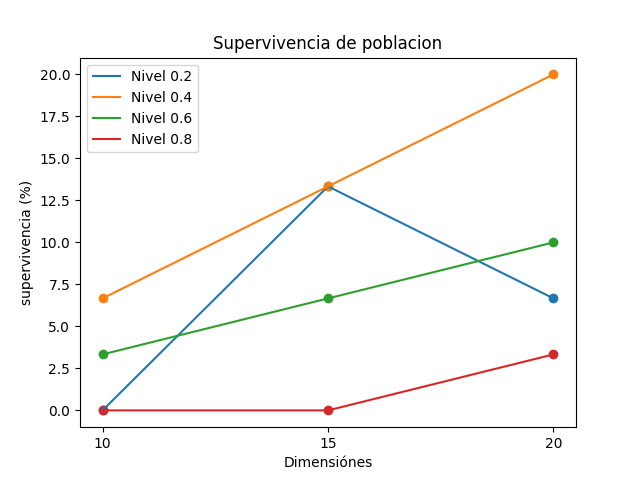
\includegraphics[width=100mm]{IMAGENES/Figure_1.png}
        \caption{Gráfica tomada del repositorio de Raul L. del código de Python 
    \url{https://https://github.com/Raullr28/Resultados/blob/main/P2/Figure_1.png}}
     \label{}
 \end{figure}
 
 % Tabla 1 
 \begin{table}[h]
 \caption{Porcentajes obtenidos del valor 0.2 (color azul) }
\centering
\begin{tabular}{ |p{2cm}||p{2cm}|p{2cm}|p{2cm}|p{2cm  }|}
 \hline
 Dimensión & Vivos & Porcentaje de vivos & Muertos & Porcentaje de muertos \\
 \hline
 10   & 1      & 3.33333 & 29      & 26.66666\\
 15   & 7      & 23.3333 & 23      & 76.66666\\
 20   & 1      & 3.3333  & 29      & 26.66666\\
 
 \hline
\end{tabular}
\label{table:1}
\end{table}

 % Tabla 2 
 \begin{table}[h]
 \caption{Porcentajes obtenidos del valor 0.4 (color naranja)}
\centering
\begin{tabular}{ |p{2cm}||p{2cm}|p{2cm}|p{2cm}|p{2cm  }|}
\hline
 Dimensión & Vivos & Porcentaje de vivos & Muertos & Porcentaje de muertos \\
 \hline
 10   & 0      & 0.0 & 30      & 1000.0\\
 15  & 1      & 3.3333  & 29      & 26.66666\\
 20   & 6      & 20  & 24      & 80 \\
 \hline
\end{tabular}
\label{table:1}
\end{table}
 
 % Tabla 3 
 \begin{table}[h]
 \caption{Porcentajes obtenidos del valor 0.6 (color verde)}
\centering
\begin{tabular}{ |p{2cm}||p{2cm}|p{2cm}|p{2cm}|p{2cm  }|}
\hline
Dimensión & Vivos & Porcentaje de vivos & Muertos & Porcentaje de muertos \\
 \hline
 10  & 0     & 0.0      & 30   &     1000.0\\
 15  & 2     & 6.66666  & 28   &     93.33333\\
 20  & 8     & 26.66666 & 20   &     73.33333 \\
 \hline
 
\end{tabular}
\label{table:1}
\end{table}
 
  % Tabla 4
 \begin{table}[h]
 \caption{Porcentajes obtenidos del valor 0.8 (color rojo)}
\centering
\begin{tabular}{ |p{2cm}||p{2cm}|p{2cm}|p{2cm}|p{2cm  }|}
 \hline
Dimensión & Vivos & Porcentaje de vivos & Muertos & Porcentaje de muertos \\

 \hline
 10  & 1      & 3.3333  & 29      & 26.66666\\
 15  & 0     & 0.0      & 30   &     1000.0\\
 20  & 0     & 0.0      & 30   &     1000.0 \\
 \hline
 
\end{tabular}
\label{table:1}
\end{table}
 
 \newpage
 

 \section{Conclusión}

 Se realiz\'{o} la segunda tarea correctamente, obteniendo una gráfica donde se observa el comportamiento de los diferentes niveles con un valor de 0.2, 0.4, 0.6 y 0.8 contra el porcentaje de supervivencia, el cual muestra ser un porcentaje muy bajo de población viva al final de todos los recorridos.
 
 Con ello se demuestra que el valor con menos población viva fue el de el nivel más grande (0.8), en este caso se volvió a realizar el experimento con una repeteción más grande, lo que generó una población igual de pequeña que con la repetición de 30.
 
 De esta forma, se demostró que los niveles más pequeños tienen más probabilidad de tener una mayor población, al ser comparados con los niveles más grandes, en los cuales no importa si hay más repeticiones o menos repeticiones, su población es casi nula.\citep{ejemplo2}
 
 

 \bibliography{biblio.bib}
 \bibliographystyle{plainnat}

 \end{document}


